\documentclass[a4paper,20pt]{article}
\usepackage{amsmath,amssymb,epsf,epsfig,times}
\usepackage{multicol}
\usepackage[all]{xy}
\usepackage{color}
\usepackage{ctex}
\usepackage{subfigure}
\usepackage{url,cite}
\usepackage{tikz}
\usepackage[english]{babel}
\usepackage[utf8]{inputenc}

\usepackage{pdfpages}

%\usepackage{caption}
%
%\usepackage[font=small,labelfont=bf,labelsep=none]{caption}
\usepackage[font=default,labelfont=bf,labelsep=period]{caption}

\usepackage{makecell}
\usepackage{booktabs} %引入三线表
\usepackage{diagbox}
\usepackage{multirow}

\usepackage{fancyhdr}
\usepackage{float}
\usepackage{ulem}

\usepackage{listings}
\usepackage{xcolor}

\usepackage{enumerate}
\lstset{
    basicstyle          =   \sffamily,          % 基本代码风格
    keywordstyle        =   \bfseries,          % 关键字风格
    commentstyle        =   \rmfamily\itshape,  % 注释的风格,斜体
    stringstyle         =   \ttfamily,  % 字符串风格
    flexiblecolumns,                % 别问为什么,加上这个
    numbers             =   left,   % 行号的位置在左边
    showspaces          =   false,  % 是否显示空格,显示了有点乱,所以不现实了
    numberstyle         =   \zihao{-5}\ttfamily,    % 行号的样式,小五号,tt等宽字体
    showstringspaces    =   false,
    captionpos          =   t,      % 这段代码的名字所呈现的位置,t指的是top上面
    frame               =   lrtb,   % 显示边框
}
\lstdefinestyle{Python}{
    language        =   Python, % 语言选Python
    basicstyle      =   \zihao{-5}\ttfamily,
    numberstyle     =   \zihao{-5}\ttfamily,
    keywordstyle    =   \color{blue},
    keywordstyle    =   [2] \color{teal},
    stringstyle     =   \color{magenta},
    commentstyle    =   \color{red}\ttfamily,
    breaklines      =   true,   % 自动换行,建议不要写太长的行
    columns         =   fixed,  % 如果不加这一句,字间距就不固定,很丑,必须加
    basewidth       =   0.5em,
}

\newtheorem{theorem}{Theorem}[section]
\newtheorem{lemma}{Lemma}[section]
\def\proof{\noindent{\it Proof: }}
\def\QED{\mbox{\rule[0pt]{1.5ex}{1.5ex}}}
\def\endproof{\hspace*{\fill}~\QED\par\endtrivlist\unskip}
\newcommand{\re}{\mathbb{R}}
\def\sV{\mathcal{V}}
\def\sS{\mathcal{S}}
\def\sQ{\mathcal{Q}}

\newcommand{\mc}{\mbox{: }}

\newcommand{\normsq}[1]{\left\|#1\right\|^2}
\newcommand{\norm}[1]{\left\|#1\right\|}
%\newcommand{\sgn}[1]{\mbox{sgn}(#1)}
\newcommand{\pde}[2]{\frac{\partial #1}{\partial #2}}
\newcommand{\fundef}[3]{#1:#2\to #3}
\newcommand{\abs}[1]{\left|#1\right|}
\newcommand{\mymatrix}[2]{\left(\begin{array}{#1}#2\end{array}\right)}
\newcommand{\defeq}{\stackrel{\triangle}{=}}
\newcommand{\paren}[1]{\left(#1\right)}
%\theoremstyle{plain} \newtheorem{theorem}{Theorem}
%\theoremstyle{plain} \newtheorem{algorithm}{Algorithm}
\newtheorem{axiom}[theorem]{Axiom}
\newtheorem{definition}[theorem]{Definition}
\newtheorem{assumption}[theorem]{Assumption}
\newtheorem{example}[theorem]{Example}
%\theoremstyle{plain}\newtheorem{lemma}{Lemma}
%\newtheorem{proposition}[theorem]{Proposition}
\newtheorem{remark}[theorem]{Remark}
\newtheorem{corollary}[theorem]{Corollary}

\newcommand{\Acal}{\mathcal{A}}
\newcommand{\Bcal}{\mathcal{B}}
\newcommand{\Ccal}{\mathcal{C}}
\newcommand{\Dcal}{\mathcal{D}}
\newcommand{\Ecal}{\mathcal{E}}
\newcommand{\Fcal}{\mathcal{F}}
\newcommand{\Gcal}{\mathcal{G}}
\newcommand{\Hcal}{\mathcal{H}}
\newcommand{\Ical}{\mathcal{I}}
\newcommand{\Jcal}{\mathcal{J}}
\newcommand{\Kcal}{\mathcal{K}}
\newcommand{\Lcal}{\mathcal{L}}
\newcommand{\Mcal}{\mathcal{M}}
\newcommand{\Ncal}{\mathcal{N}}
\newcommand{\Ocal}{\mathcal{O}}
\newcommand{\Pcal}{\mathcal{P}}
\newcommand{\Qcal}{\mathcal{Q}}
\newcommand{\Rcal}{\mathcal{R}}
\newcommand{\Scal}{\mathcal{S}}
\newcommand{\Tcal}{\mathcal{T}}
\newcommand{\Ucal}{\mathcal{U}}
\newcommand{\Vcal}{\mathcal{V}}
\newcommand{\Wcal}{\mathcal{W}}
\newcommand{\Xcal}{\mathcal{X}}
\newcommand{\Ycal}{\mathcal{Y}}
\newcommand{\Zcal}{\mathcal{Z}}


\def\omegavec{\boldsymbol{\omega}}
\newcommand{\alphabf}{\boldsymbol{\alpha}}
\newcommand{\omegabf}{\boldsymbol{\omega}}
\def\omegavec{\boldsymbol{\omega}}
\newcommand{\taubf}{\boldsymbol{\tau}}
\newcommand{\qbf}{\mathbf{q}}
\newcommand{\ybf}{\mathbf{y}}
\newcommand{\pbf}{\mathbf{p}}
\newcommand{\rbf}{\mathbf{r}}
\newcommand{\ebf}{\mathbf{e}}
\newcommand{\onebf}{\mathbf{1}}
\newcommand{\zerobf}{\mathbf{0}}
\newcommand{\abf}{\mathbf{a}}
\newcommand{\ibf}{\mathbf{i}}
\newcommand{\jbf}{\mathbf{j}}
\newcommand{\kbf}{\mathbf{k}}
\newcommand{\vbf}{\mathbf{v}}
\newcommand{\wbf}{\mathbf{\omega}}
\newcommand{\fbf}{\mathbf{f}}
\newcommand{\zbf}{\mathbf{z}}
\newcommand{\xbf}{\mathbf{x}}
\newcommand{\dbf}{\mathbf{d}}
\newcommand{\Rbf}{\mathbf{R}}
\newcommand{\Tbf}{\mathbf{T}}

\newcommand{\Cbf}{\mathbf{C}}
\newcommand{\Ibf}{\mathbf{I}}
\newcommand{\Pbf}{\mathbf{P}}
\newcommand{\Qbf}{\mathbf{Q}}
\newcommand{\Vbf}{\mathbf{V}}
\newcommand{\Jbf}{\mathbf{J}}
\newcommand{\Xbf}{\mathbf{X}}
\newcommand{\Abf}{\mathbf{A}}
\newcommand{\Kbf}{\mathbf{K}}
\newcommand{\Gammabf}{\boldsymbol{\Gamma}}
\newcommand{\nubf}{\boldsymbol{\nu}}
\newcommand{\xibf}{\boldsymbol{\xi}}
\newcommand{\Xibf}{\boldsymbol{\Xi}}
\newcommand{\Omegabf}{\boldsymbol{\Omega}}


\newcommand{\ubf}{\mathbf{u}}

\newcommand{\lth}{\ell{\text{th}}}
\newcommand{\ith}{i{\text{th}}}
\newcommand{\jth}{j{\text{th}}}
\newcommand{\kth}{k{\text{th}}}
\newcommand{\ip}[2]{\left<#1,~#2\right>}

\newcommand{\OMIT}[1]{}
\title{}
\author{}
\date{}


\pagestyle{fancy}
\fancyhf{}
\chead{\textbf{关于$\lceil$\textcolor{red}{“非线性规划”}$\rfloor$的matlab讲解}}
\lhead{魔力铠甲}
\rfoot{Page \thepage}
\begin{document}
\renewcommand{\lstlistlistingname}{代码汇总}
\renewcommand{\lstlistingname}{代码}
\captionsetup[figure]{labelfont={bf},labelformat={default},labelsep=period,name={图}}
\renewcommand\tablename{表}
好的,我们来到第三篇。规划类问题就快要完结了。推荐与运筹学结合起来一起学习。
\section{非线性规划-简介}
如果目标函数或约束条件中包含非线性函数,就称这种规划问题为非线性规划问
题。
\par \textbf{八股文:}根据约束条件的不同,我们将非线性规划分为无约束线性规划问题(以下记作:F)和有约束线性规划问题(以下记作:T),其中有约束问题就是至少有一个约束条件的非线性规划问题。由于现在没有一种算法保证可以找出任何的全局最优解,通常我们只能找到算法的局部最优解。
\subsection{有限的条件下,最大的收益}
求下列非线性规划
$\min f(x) = x_1^2+x_2^2+x_3^2+8$
\\s.t.$\left\{\begin{matrix}
        x_1^2-x_2+x_3^2 \geqslant 0  \\
        x_1+x_2^2+x_3^2 \leqslant 20 \\
        -x_1-x_2^2+2=0               \\
        x_2+x_3^2=3                  \\
        x_1,x_2,x_3\geqslant 0       \\
    \end{matrix}\right.$
\par \small{解:} \\
\fbox{%
    \parbox{\textwidth}{%
        \begin{center}

            目标函数 $\min f(x) = x_1^2+x_2^2+x_3^2+8$
            \\同时给出约束条件
            \\s.t.$\left\{\begin{matrix}
                    x_1^2-x_2+x_3^2 \geqslant 0  \\
                    x_1+x_2^2+x_3^2 \leqslant 20 \\
                    -x_1-x_2^2+2=0               \\
                    x_2+x_3^2=3                  \\
                    x_1,x_2,x_3\geqslant 0       \\
                \end{matrix}\right.$
        \end{center}

    }%
}
\par \noindent \large \textcolor{blue}{给出matlab调用函数fmincon函数的解法的模型化:}
\par \noindent matlab给出的数学模型如下:
\\ $\min Z = f(x)$
\\s.t.$\left\{\begin{matrix}
        Ax\leq b   \\
        Aeqx = beq \\
        C(x)\leq 0 \\
        Ceq(x) = 0 \\
    \end{matrix}\right.$
\par 其中 $f (x)$是标量函数, $A, B, Aeq, Beq$是相应维数的矩阵和向量,$C(x),Ceq(x)$ 是非
线性向量函数。
\par 接下来给出我们最常用的matlab代码形式:
\begin{center}
    X=FMINCON(FUN,X0,A,B,Aeq,Beq,LB,UB,{NONLCON},{OPTIONS})
\end{center}
更加详细一点:
\\它的返回值是向量 x ,
\\其中 FUN 是用 M 文件定义的函数 f (x);X0 是 x 的初始值;
\\A,B,Aeq,Beq 定义了线性约束 A* X ≤ B, Aeq * X = Beq ,如果没有线性约束,则A=[],B=[],Aeq=[],Beq=[];
\\LB 和 UB 是变量 x 的下界和上界,如果上界和下界没有约
束,则 LB=[],UB=[],如果 x 无下界,则 LB 的各分量都为-inf,如果 x 无上界,则 UB
的各分量都为 inf;
\\NONLCON 是用 M 文件定义的非线性向量函数C(x),Ceq(x) ;
\\OPTIONS定义了优化参数,可以使用 Matlab 缺省的参数设置。

\par \noindent  \textbf{\textcolor{red}{特殊情况:}}求解二次规划的函数quadprog,目标函数是非线性的,但是约束条件是线性函数,这样的非线性规划我们叫做二次规划。
\par 求解二次规划:
\par \noindent
\fbox{
    \parbox{\textwidth}{
        目标函数$\min f(x)=2x_1^2-4x_1x_2+4x_2^2-6x_1-3x_2$
        \\$f(x)=$
            \\同时给出约束条件
            \\s.t.$\left\{ \begin{matrix}
            x_1+x_2 \leq 3  \\
            4x_1+x_2 \leq 9 \\
            x_1,x_2\geq 0
        \end{matrix} \right.$}
}
\par \noindent \textcolor{blue}{给出matlab调用函数quadprog函数的解法的模型化}
\par \noindent matlab给出的数学模型如下:
\\$\min Z=\frac{1}{2}x^THx+f^Tx$
    \\s.t.$\left\{\begin{matrix}
    Ax\leq b         \\
    Aeq\cdot x = beq \\
\end{matrix} \right.$
    \par 其中H 是实对称矩阵, f ,b 是列向量, A 是相应维数的矩阵。
    \par 接下来给出我们最常用的matlab代码形式:
    \begin{center}
        $\left[X,\text{FVAL}\right]$= QUADPROG(H,f,A,b,Aeq,beq,LB,UB,X0,OPTIONS)
    \end{center}
    其中H是一个正定矩阵(如果要求有限最小值);f是化为二次型后剩余的函数;
    \\A,b,Aeq,beq分别是线性约束,如没有,用'[]'代替。
    \\LB,UB分别为上下界,若无则'[]',若无穷则可设'-inf''inf'。
    \\x0是x的初始值;OPTIONS定义了相关优化参数。
    \section{非线性规划-适用题目}
    \subsection{非线性规划适用的赛题:}
    题目中提到"怎样安排/分配”"尽量多(少)” “最多(少)” "利润最大” “最合理” 等词;但变量非一次方
    \begin{itemize}
        \item[·\textcolor{blue}{生产安排}] 原材料、设备有限制,总利润最大(目标函数或约束条件非线性)
            生产两种机床,利润分别为XXX, A机器和B机器加工,两种机器工作时间…;成本或利润与某变量的关系是非线性的
        \item[·\textcolor{blue}{选址问题}] 已知新建工厂位置,各工地需求量,当前工厂货物需求量,各种距离的单位运输量,新工厂建在何地是单位运输量最大。
        \item[·\textcolor{blue}{角度调整}] 飞行管理避免相撞; 影院最佳视角
            飞机位置,速度,进入区域后判定是否相撞, 飞机飞行方向角调整的幅度尽量小
            电影院视角、仰角影响观影体验,什么位置观影最佳涉及三角函数,为非线性规划。
    \end{itemize}
    \subsection{模型假设}
    无约束非线性规划问题:在 Matlab 中,用于求解无约束最值问题的函数有 fminunc 和 fminsearch,
    来求函数的极小值$\min\limits_x f(x)$。
    \par 1.matlab中无约束条件多变量求最小值fminunc用法为:
    \begin{center}
        $\left[x,fval\right]$=fminunc(FUN,$x_0$,OPTIONS,P1,P2, ...)
    \end{center}
    \par \noindent 更加详细一点:
    \\它的返回值 x是极小值点 , fval是求得的极小值,以及还有其他未列出的返回值。
    \\其中 FUN 是用 M 文件定义的函数 f (x);X0 是 x 的初始值;
    \\当FUN文件只有一个返回值时,它返回的是函数$f(x)$;当它有两个返回值时,返回的是梯度向量;当它有三个返回值时,返回的是二阶导Hessian矩阵。
    \\这个时候,fminunc的写法是:
    \begin{center}
        \par \noindent $\left[x,fval,\text{exitflag},\text{output},\text{grad},\text{hessian}\right]$  = fminunc(\_\_\_)
        \\返回描述 fminunc 的退出条件的值 exitflag,以及提供优化过程信息的结构体 output。
    \end{center}
    \par \noindent OPTIONS定义了优化参数,可以使用 Matlab 缺省的参数设置。
    \par \textbf{例:}
    \par \noindent \fbox{
        \parbox{\textwidth}{
            编写返回极小值点和极小值的目标函数。使用包括梯度和 Hessian 矩阵 中所述的条件化形式。目标函数是 Rosenbrock 函数,
            $$f(x)=100(x_2-x_1^2)^2+(1-x_1^2)^2$$
            它有梯度$\nabla f(x)=\begin{bmatrix}
                    -400(x_2-x_1^2)^2x_1-2(1-x_1) \\
                    200(x_2-x_1^2)                \\
                \end{bmatrix}$
            \\它有海森矩阵$H(x)=\begin{bmatrix}
                    12x^2-400y+2 & -400x \\
                    -400x        & 20000 \\
                \end{bmatrix}$        }
    }
    \par \noindent \textbf{可以给出梯度法的代码如下:}
    \begin{center}
        \begin{lstlisting}[caption={Fminunc\_1},language=Matlab]
% NonLinear Programming
        %This is Obejctive1.m
function [f,g]=Objective1(x) 
f=100*(x(2)-x(1)^2)^2+(1-x(1))^2; 
g=[-400*x(1)*(x(2)-x(1)^2)-2*(1-x(1));200*(x(2)-x(1)^2)];
        %This is Example1.m
options = optimset('GradObj','on');
[x,y] = fminunc('Objective1',rand(1,2),options)
%x =    1.0000    1.0000
%y =    3.6009e-15
        \end{lstlisting}
    \end{center}
    \par \noindent \textbf{可以给出Hessan矩阵法的代码如下:}
    \begin{center}
        \begin{lstlisting}[caption={Fminunc\_2},language=Matlab]
% NonLinear Programming
        %This is Objective2.m
function [f,df,d2f]=Objective2(x)
f=100*(x(2)-x(1)^2)^2+(1-x(1))^2; 
df=[-400*x(1)*(x(2)-x(1)^2)-2*(1-x(1));200*(x(2)-x(1)^2)]; 
d2f=[-400*x(2)+1200*x(1)^2+2,-400*x(1) 
 -400*x(1),200];
        %This is Example2.m
options = optimset('GradObj','on','Hessian','on');
[x,y]=fminunc('Objective2',rand(1,2),options)
%x =   1.0000    1.0000
%y =   8.4869e-24
        \end{lstlisting}
    \end{center}

    \par 2.matlab中无导数无约束条件多变量求最小值fminsearch用法为:
    \begin{center}
        $\left[x,fval\right] $=fminunc(fun,x0,options)
    \end{center}
    \par \noindent 更加详细一点:
    \\它的返回值 x是极小值点,fval是求得的极小值,以及还有其他未列出的返回值。
    \\其中 FUN 是用M文件定义的函数f(x);x0是x的初始值;
    \\可以添加exitflag与output来分别输出退出条件的值与和优化过程有关的信息。
    \\这个时候,fminunc的写法是:
    \begin{center}
        \par \noindent $\left[x,fval,exitflag,output \right]$= fminsearch(\_\_\_)
    \end{center}
    \par \textbf{例:}
    \par \noindent \fbox{
    \parbox{\textwidth}{
    将起始点设置为 x0 = [-1.2,1] 并使用 fminsearch 计算 Rosenbrock 函数的最小值。目标函数是 Rosenbrock 函数,
    $$f(x)=100(x_2-x_1^2)^2+(1-x_1^2)^2$$
    该函数的最小值在 x = [1,1] 处,最小值为 0。
    }
    }
    \par \noindent \textbf{可以给出fminsearch代码如下:}
    \begin{center}
        \begin{lstlisting}[caption={fminsearch},language=Matlab]
% NonLinear Programming
        %This is Objective3.m
function result = Objective3(x)
    result = 100*(x(2) - x(1)^2)^2 + (1 - x(1))^2;
end
        %This is Example3.m
options = optimset('PlotFcns',@optimplotfval);
x0 = [-1.2,1];
x = fminsearch(@Objective3,x0,options)
%x =    1x2    1.0000    1.0000

        \end{lstlisting}
    \end{center}
    \par \noindent 可以得到运行结果图如图1。
    \\当然,这个时候可以看出Rosenbrock函数的最小值就是[1,1]处的0值。
    \begin{center}
        \begin{figure}[H]
            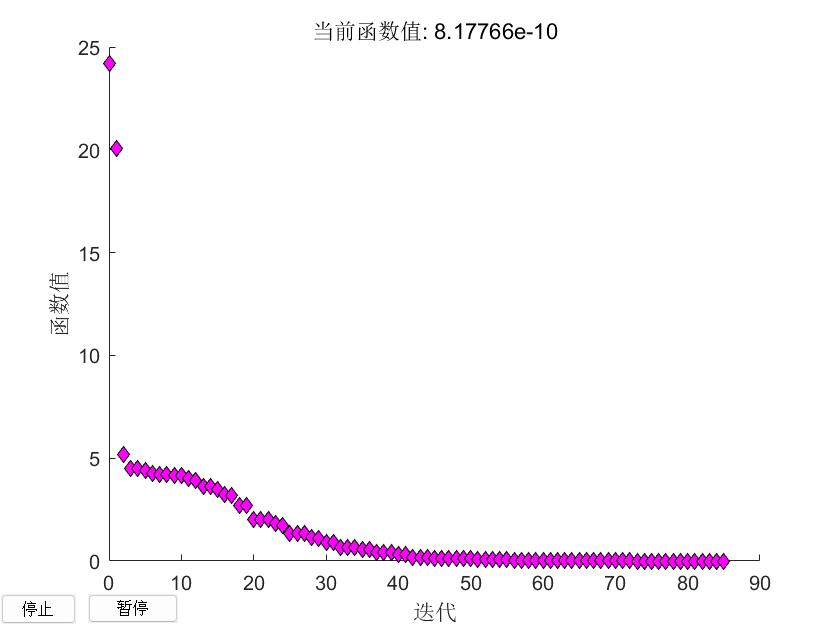
\includegraphics[width=340pt,height=195pt]{Example3.jpg}
            \caption{运行结果}
        \end{figure}
    \end{center}
    \par 在 Matlab 优化工具箱中,用于求解约束最优化问题的函数有:fminbnd、fmincon、
    quadprog、fseminf、fminimax。可以参考matlab算法大全第三章相关例题进行学习。
    \par \noindent 寻找单变量非线性函数在区间上的最小值fminbnd用法为:
    \begin{center}
        $\left[x,fval \right]$={fminbnd}({fun},{x1},{x2},{OPTIONS})
    \end{center}
    \par \noindent 更加详细一点:
    \\它的返回值x是极小值点,fval是求得的极小值,以及还有其他未列出的返回值。
    \\其中fun是用M文件定义的单变量科学函数f(x)
    \\可以添加exitflag与output来分别输出退出条件的值与和优化过程有关的信息
    \\这个时候,fminbnd的写法是:
    \begin{center}
        $\left[ \text{x,fval,exitflag,output}\right]$=fminbnd(\_\_\_)
    \end{center}
    \par \textbf{例:}
    \par \noindent \fbox{
        \parbox{\textwidth}{
            求单变量非线性函数$f(x)=(x-3)^2-1,x\in\left[0,5\right]$的极小值。
        }
    }
    \par \noindent \textbf{可以给出fminbnd代码如下:}
    \begin{center}
        \begin{lstlisting}[caption={Fminbnd},language=Matlab]
% NonLinear Programming
        %This is Objective4.m
function f = Objective4(x) 
    f=(x-3)^2-1;
end
        %This is Example4.m
[x,y]=fminbnd('Objective4',0,5) 
%x =    3     y =   -1
            \end{lstlisting}
    \end{center}
    \par \noindent 求解半无限约束多元函数的最小值fseminf用法为:
    \begin{center}
        x = fseminf(fun,x0,ntheta,seminfcon,A,b,Aeq,beq,lb,ub,options)
    \end{center}
    \par \noindent 更加详细一点:
    \\它的返回值x是极小值点。
    \\其中fun是用M文件定义的线性或非线性函数;x0是初始值点;
    \\ntheta,seminfcon是无穷半约束条件。
    \\A,b,Aeq,beq分别是A*x$\leq$b,Aeq*x=beq的约束条件;
    \\可以添加exitflag与output来分别输出退出条件的值与和优化过程有关的信息,同时还有lamdba结构体包含在解 x 处的拉格朗日乘数。
    \\这个时候,fseminf的写法是
    \begin{center}
        $\left[\text{x,fval,exitflag,output,lambda}\right]$ = fseminf(\_\_\_)
    \end{center}
    \par \textbf{例:}
    \par \noindent \fbox{
        \parbox{\textwidth}{
            求函数$f(x)=(x_1-0.5)^2+(x_2-0.5)^2+(x_3-0.5)^2$取最小值时的 x 值,约束是
            $$K_1(x,w_1)=sin(w_1x_1)cos(w_1x_2)-\frac{1}{1000}(w_1-50)^2-sin(w_1x_3)-x_3\leq 1 $$
            $$K_2(x,w_2)=sin(w_2x_2)cos(w_2x_1)-\frac{1}{1000}(w_2-50)^2-sin(w_1x_3)-x_3\leq 1 $$
            $$ 1\leq w_1 \leq 100,1\leq w_2 \leq 100$$
        }
    }
    \par \noindent \textbf{可以给出fseminf代码如下:}
    \begin{center}
        \begin{lstlisting}[caption={Fseminf},language=Matlab]
% NonLinear Programming
        %This is Objective5_1.m
function f=Objective5_1(x,s)
f=sum((x-0.5).^2);
end
        %This is Objective5_2.m
function [c,ceq,k1,k2,s]=Objective5_2(x,s)
c=[];
ceq=[];
if isnan(s(1,1))
    s=[0.2,0;0.2,0];
end
w1=1:s(1,1):100;
w2=1:s(2,1):100;
k1=sin(w1*x(1)).*cos(w1*x(2))-...
1/1000*(w1-50).^2-sin(w1*x(3))-x(3)-1;
k2=sin(w2*x(2)).*cos(w2*x(1))-...
1/1000*(w2-50).^2-sin(w2*x(3))-x(3)-1;
plot(w1,k1,'-',w2,k2,'+');
plot(w1,k1,'-',w2,k2,'+');
        %This is Example5.m
[x,y]=fseminf(@Objective5_1,rand(3,1),2,@Objective5_2)
%x =    0.9170      1.0123      0.1481
%y =     0.5602
            \end{lstlisting}
    \end{center}
    \par \noindent 寻找能够最小化一组目标函数最大值的点的fminimax用法为:
    \begin{center}
        x=fminimax(FUN,x0,A,b,Aeq,beq,lb,ub,OPTIONS)
    \end{center}
    \par \noindent 更加详细一点:
    \\它的返回值x是一组使函数族最大的极小值点。
    \\其中fun是用M文件定义的线性或非线性函数族;x0是初始值点;
    \\ntheta,seminfcon是无穷半约束条件。
    \\A,b,Aeq,beq分别是A*x$\leq$b,Aeq*x=beq的约束条件;
\\可以添加exitflag与output来分别输出退出条件的值与和优化过程有关的信息,同时还有lamdba结构体包含在解 x 处的拉格朗日乘数。
\\这个时候,fseminf的写法是
\begin{center}
    $\left[\text{x,fval,maxfval,exitflag,output,lambda}\right]$ = fminimax(\_\_\_)
\end{center}
\par \textbf{例:}
\par \noindent \fbox{
    \parbox{\textwidth}{
        求函数族\{$f_1(x),f_2(x),f_3(x),f_4(x),f_5(x)$\}取极大极小值时的x值。其中:
        $\left\{\begin{matrix}
                f_1(x)=2x_1^2+x_2^2-48x_1-40x_2+304 \\
                f_2(x)=-x_1^2-3x_2^2                \\
                f_3(x)=x_1+3x_2-18                  \\
                f_4(x)=-x_1-x_2                     \\
                f_5(x)=x_1+x_2-8                    \\
            \end{matrix}\right.$
    }
}
\par \noindent \textbf{可以给出fminimax代码如下:}
\begin{center}
    \begin{lstlisting}[caption={fminimax},language=Matlab]
% NonLinear Programming
        %This is Objective6.m
function f=Objective6(x)
f=[2*x(1)^2+x(2)^2-48*x(1)-40*x(2)+304
    -x(1)^2-3*x(2)^2
    x(1)+3*x(2)-18
    -x(1)-x(2)
    x(1)+x(2)-8];
end
        %This is Example6.m
[x,y]=fminimax(@Objective6,rand(2,1))
%x =    4.0000    4.0000
%y =    0.0000  -64.0000   -2.0000   -8.0000   -0.0000
            \end{lstlisting}
\end{center}
\section{非线性规划-代码实现}
\par 贴出matlab代码求解,请对应相应的函数。
\begin{center}
    \begin{lstlisting}[caption={Fmincon},language=Matlab]
% NonLinear Programming
        %This is fun1.m
function f=fun1(x)
f=sum(x.^2)+8;
end
        %This is fun2.m
function [g,h]=fun2(x)
g=[-x(1)^2+x(2)-x(3)^2 
x(1)+x(2)^2+x(3)^3-20]; %Nonlinear inequality constraints 
h=[-x(1)-x(2)^2+2 
x(2)+2*x(3)^2-3]; %Nonlinear equality constraints
        %This is example.m
options=optimset('largescale','off'); 
[x,y]=fmincon('fun1',rand(3,1),[],[],[],[],zeros(3,1),[], ... 
'fun2', options) 
        \end{lstlisting}
\end{center}
\begin{center}
    \begin{lstlisting}[caption={Quadprog},language=Matlab]
    % NonLinear Programming
            %This is subexample.m
    h=[4,-4;-4,8]; 
    f=[-6;-3]; 
    a=[1,1;4,1]; 
    b=[3;9]; 
    [x,value]=quadprog(h,f,a,b,[],[],zeros(2,1)) 
    %x =    1.9500     1.0500    value =    -11.0250
            \end{lstlisting}
\end{center}

\section{非线性规划-实战演练}
非线性规划可以说是国赛里面很容易考的问题,因为matlab也没有固定的算法能够很好地解决NLP问题。所以非线性规划目前还没有适于各种问题的一般算法,各个方法都有自己特定的适用范围。
这样也让出题人有了一定的操作空间。这章讲了非线性规划,结束,收工。
\newpage
\begin{thebibliography}{99}

    \bibitem{ref1}谢中华. MATLAB与数学建模[A].北京航空航天大学出版社[M]:科学技术协会,2021-02-14.
    \bibitem{ref2}数学建模BOOM. 【数模美赛国赛】非线性规划(模型+适用赛题+MATLAB求解,数学建模零基础入门))[M]:2021-08-30.
    \bibitem{ref3}mathworks. 非线性规划问题求解器[J]:\url{https://ww2.mathworks.cn/help/optim/ug/linprog.html#description}
    \bibitem{ref4}mathworks. 求无约束多变量函数的最小值--fminunc[J]:\url{https://ww2.mathworks.cn/help/optim/ug/fminunc.html#d124e57611}
    \bibitem{ref5}mathworks. 寻找约束非线性多变量函数的最小值--fmincon[J]:\url{https://ww2.mathworks.cn/help/optim/ug/fmincon.html}
    \bibitem{ref6}mathworks. 使用无导数法计算无约束的多变量函数的最小值--fminsearch[J]:\url{https://ww2.mathworks.cn/help/matlab/ref/fminsearch.html}
    \bibitem{ref7}VL\_L\_\^\_\^. 数学建模-影院角度[M].\url{https://www.cnblogs.com/Lovely-Boy/p/12828814.html},2020-05-04.
    \bibitem{ref8}飘渺到放弃.[学习笔记]非线性规划实例——飞行管理问题[M].\url{https://blog.csdn.net/weixin_46059493/article/details/106164593},2020-05-16
    % \bibitem{ref2}陈香敏,魏伟,吴莹. “文化+人工智能”视阈下文化创意产业融合发展实践及路径研究[A]. 中共沈阳市委、沈阳市人民政府.第十七届沈阳科学学术年会论文集[C].中共沈阳市委、沈阳市人民政府:沈阳市科学技术协会,2020:4.
    % \bibitem{ref3}田晓曦,刘振鹏,彭宝权. 地方高校开展教育人工智能深度融合的路径探究[A]. 中共沈阳市委、沈阳市人民政府.第十七届沈阳科学学术年会论文集[C].中共沈阳市委、沈阳市人民政府:沈阳市科学技术协会,2020:5.
    % \bibitem{ref4}柏卓君,潘勇,李仲余.彩色多普勒超声在早期胚胎停育诊断中的应用[J].影像研究与医学应用,2020,4(18):129-131.
    % \bibitem{ref5}杨芸.我院2018年人血白蛋白临床应用调查与分析[J].上海医药,2020,41(17):34-35+74.

\end{thebibliography}
\newpage
\section{数学建模算法大全第三章习题答案}
\begin{itemize}
    \item[1.] 给出梯度最速下降法的解,代码详见homework1.m与deltaf.m:
        \\$ x =\qquad   0.3333 \qquad 1.3333$    \\$Z =\qquad  4.6667$
    \item[2.] 编码请看Homework2.m与nwfun.m.(此时步长为1)
        \\极值点是$x=0,y=0$
        \\极值是$Z=-0.5$(共迭代408次)
        \\另一个编码请看c\_gradientDescent.m(此时步长可变)
        \\极值点是$ x=10^{-4}*0.1002,y=0$(迭代100次左右)
        \\极值是$Z=-0.5$(迭代59次左右)
    \item[3.]   数学模型为:
        \par \noindent $\min f(x)=0.2(x_1^2+x_2^2+x_3^2)+58x_1+54x_2+50x_3-560$
        \\s.t.$\left\{\begin{matrix}
                x_1+x_2+x_3=180    \\
                x_1+x_2\geq 100    \\
                x_1 \geq 40        \\
                x_1,x_2,x_3 \geq 0 \\
            \end{matrix} \right.$
        \\给出非线性规划的解:   $x_1=50
            \quad x_2=60
            \quad x_3=70$
        \\$fval =1.0160*10^{4}$
    \item[4.] 给出解,代码详见homework4.m,Objfun41.m与Confun41.m
        \\$x =\quad  0.0000  \quad  0.0000  \quad  2.7977 \quad  -0.0001  \quad  0.0000  \quad  0.9321$
    \item[5.] 解同4,留给读者。
    \item[6.] 给出fmincon的解,代码详见homework6.m,Objfun61.m与Objfun62.m:
        \\$x =\qquad    2.3333 \qquad   0.1667 \qquad  -3.4444$
            \\$fval =\qquad  18.0833 $
        \item[7.]给出matlab建模的解:
        \\代码详见homework7\_1.m,homework7\_2.m,homework7\_3.m:
        \par \noindent (1) 距离屏幕大概6.211m处(第三或第四排)。
        \par \noindent (2)  $20^\circ$时,观众满意度最大。
        \par \noindent (3) 可以改成y关于x的二次曲线($y=-0.0073*x^2+0.1618x+4.1940$),然后取a,b,c使得$\alpha$最大
\end{itemize}
\end{document}